{
\newcommand\myrect[5]{\draw (#1,#2) rectangle ({#1+#3},{#2+#4}) node[pos=0.5] {#5} ; }
\newcommand\minicipher[3]{
	\myrect{#1}{#2}{1}{1}{#3}
    \draw (#1+1, #2+0.3) -- (#1+1-0.15, #2+0.5) -- (#1+1, #2+1-0.3) ;
}

\begin{figure}[htb]
  \centering
  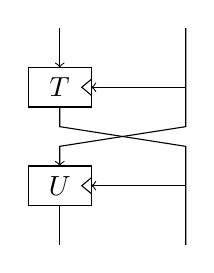
\begin{tikzpicture}[xscale=0.8, yscale=-0.5]
	\if0
	    \draw[help lines,dotted] (-2,-3) grid (2,3);
		\foreach \x in {-2,-1,0,1,2}
		    \draw (\x cm,-1pt) node[anchor=north] {\color{gray} \tiny $\x$};
		\foreach \y in {-3,-2,-1,1,2,3}
		    \draw (+3pt,\y-0.05) node[anchor=east] {\color{gray} \tiny $\y$};
	\fi

    % Mini block ciphers
	\minicipher{-1.5}{-2}{$T$}
	\minicipher{-1.5}{+0.5}{$U$}

    \draw [->] (-1,-3) -- (-1,-2);
    \draw      (-1,-1) -- (-1,-0.5) -- (1,0) -- (1,2.5);
	\draw [->] (1,1) -- (-0.5,1);

	\draw [->] (1,-3) -- (1,-0.5) -- (-1,0) -- (-1,0.5);
	\draw [->] (1,-1.5) -- (-0.5,-1.5);
	\draw      (-1,1.5) -- (-1,2.5);
  \end{tikzpicture}
  \FigDef{tu}{TU-decomposition of $\pi_2$.}
\end{figure}
}